%!TEX root = ../main.tex

\chapter{動的計画モデル}
第3章で述べた線形計画法は厳密解を得る上で強力であるが，
計画期間が長期化した場合，変数および制約条件の数が膨大となり，計算負荷が増大する可能性がある．
一方で，本研究のような蓄電池運用問題は，ある時刻(期)の状態（蓄電池の残量）と行動（蓄電池の充放電量をいかほどにするか）が決まれば，
過去の履歴に関わらず次の期の状態が決定するという性質を有している．
このような問題においては，動的計画法の適用が有効である．動的計画法は，Bellmanの最適性の原理
に基づき，問題を時間ステップごとの部分問題に分割して再帰的に解く手法である．
本手法の最大の利点は，目的関数や制約条件が非線形・不連続であっても適用可能である点，
および計算時間が計画期間$K$に対して線形に増加するため，
長期間の計画に対しても計算時間の見通しが良い点にある．本章では，蓄電池状態を離散化することで動的計画モデルを構築し，
線形計画モデルとは異なるアプローチでのモデル化を行う．

\section{本モデルでの時間の扱い}
線形計画モデルと同様，計画対象となる期間の先頭の時刻を時刻0とし，当該期間を等間隔に$K$個の区間に分割する．図\ref{fig:time_dig_dp}は
図\ref{fig:time_dig_lp}を再掲したものである．
\begin{figure}[h]
	\centering
 	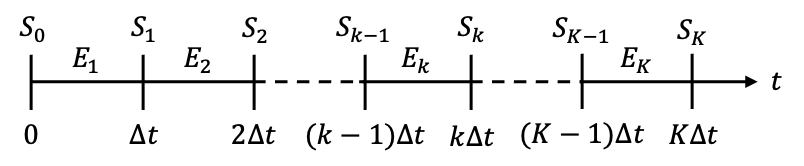
\includegraphics[width=155mm]{../figure/time_dig.png}
 	\caption{Period and measured time (aforementioned)}
 	\label{fig:time_dig_dp}
\end{figure}

\section{本モデルでの状態と行動，状態遷移関数の扱い}
	蓄電池の残量としてとりうる値を，0が最小値， $\overline{b}^{\rm F}$が最大値となるよう，等間隔に $B( \geq 2)$段階で離散化する．これにより， $k$期の末尾における	
	残量 $b_k^{\rm F}$は
	$0,\ \frac{1}{B-1}\overline{b}^{\rm F},\ \frac{2}{B-1}\overline{b}^{\rm F},\ \dots,\ \overline{b}^{\rm F}$のいずれかをとる．
	蓄電池の刻み幅$\Delta b^{\rm F}$を$\Delta b^{\rm F} = \frac{\overline{b}^{\rm F}}{B-1}$と定義する．この定義により蓄電池の残量としてとりうる値は
	$0,\Delta b^{\rm F},2\Delta b^{\rm F},\ \dots,(B-1)\Delta b^{\rm F}$
	と表される．
	また，集合$S_{0},S_{1},\ldots,S_{K}$を以下のように定義する：
	\begin{gather}
	S_k =  \{  s_0 \} ,\quad  k = 0 \\
	S_k = \{ 0, 1, \dots, B - 1 \} ,\quad  k  = 1, \ldots , K．
	 \label{eq:state}
	\end{gather}

	このもとで，集合$S_k$の要素である$s_k$は以下の条件を満たしているものと定義する：
	\begin{equation}
	b_k^{\rm F} = s_k \Delta b^{\rm F}  ,\quad  k  = 0, \ldots , K．
	\label{eq:B_K}
	\end{equation}
	以降，この整数値 $s_k$ を「蓄電池の残量の状態」と呼ぶ．

	電力運用は，各状態における意思決定と，それに伴う状態遷移の繰り返しにより構成される．
	本モデルにおいて，状態$s_{k-1}$で行う意思決定$a_k$を「行動」と呼ぶ．
	ある蓄電池の残量の状態からある行動を実行した際に，次の蓄電池の残量の状態へ遷移する関係を式\eqref{eq:state_transition}のように表し，関数$T$を「状態遷移関数」と呼ぶ．
	\begin{equation}
    		s_k = T(s_{k-1}, a_k) ，\quad  k  =1, \ldots , K
	\label{eq:state_transition}
	\end{equation}	
	本モデルにおける行動$a_k$は，「$k$期の末尾における残量（すなわち次の状態$s_k$）を選択すること」と定義する．
	したがって，$a_k$のとりうる値は蓄電池の残量の状態$s_k$と同様に$0, 1, \dots, B-1$のいずれかとなり，
	式\eqref{eq:state_transition}における状態遷移関数は単純に次のように表される：
	\begin{equation}
		T(s_{k-1}, a_k) = a_k，\quad  k  =1, \ldots , K.
    	\label{eq:state_transition_def}
	\end{equation}
	すなわち，本モデルでは行動$a_k$の決定がそのまま蓄電池の残量の状態$s_k$の決定となる．%この決定に伴い，両状態間の差分として充放電量が計算される．
	

\section{モデルの要素}
モデルの要素(\IS を付して記す)と定数(\IB を付して記す)，変数(\IC を付して表す)を列挙する．
第3章と異なる点として，
\begin{itemize}
	\item 線形計画モデルでは蓄電池の充電量と放電量をそれぞれ独立した非負の変数として定義していたが，
	本モデルではこれらを統合し，正負の値をとる単一の変数として扱っていること
	\item 商用電力系統買電力量が負の値もとりうること
	\item 蓄電池の残量は連続値ではなく，離散化された値をとること
	\item 蓄電池の残量を離散化したときの分割数という定数を導入していること
	\item 蓄電池の残量の状態を表す変数を導入していること
	\item 行動を表す変数を導入していること
\end{itemize}
が挙げられる．モデル中の定数・変数と電力グリッドとの関係を図\ref{fig:variables_dp}に示す．赤色の文字は決定変数，青色の文字は従属変数，緑色の文字は外生変数である．なお，
定数・変数の傍らに灰色で付記された文字は，その定数・変数が当該のケースを採用した場合にのみ現れることを表している．

\begin{itemize}
 	\item[\IS] 太陽光発電設備G
		\begin{itemize}
		 	\item[\IB] 太陽光発電電力量(変換前) $g^{\rm P1}_{k}$
  			\item[\IC] 太陽光発電電力量(変換後) $g^{\rm P2}_{k}$
		\end{itemize}	
	 \item[\IS] 電力消費機器D$^{\rm A}$
	 	\begin{itemize}
		 	\item[\IC] 電力需要量A (変換前) $d^{\rm A1}_{k}$
 			\item[\IB] 電力需要量A (変換後) $d^{\rm A2}_{k}$
		\end{itemize}
 	\item[\IS] 電力消費機器D$^{\rm B}$
	 	\begin{itemize}
		 	\item[\IC] 電力需要量B (変換前) $d^{\rm B1}_{k}$
 			\item[\IB] 電力需要量B (変換後) $d^{\rm B2}_{k}$
		\end{itemize}	
 	\item[\IS] 電力消費機器D$^{\rm C}$
	 	\begin{itemize}
		 	\item[\IC] 電力需要量C (変換前) $d^{\rm C1}_{k}$
 			\item[\IB] 電力需要量C (変換後) $d^{\rm C2}_{k}$
		\end{itemize}
 	\item[\IS] 電力消費機器（自己託送先）D$^{\rm D}$
 	\begin{itemize}
   		\item[\IB] 自己託送先が必要とする電力 $d^{\rm D}$
   		\item[\IB] 自己託送先へ託送することのインセンティブ係数 $p^{\rm D}$   
		\item[\IC] 自己託送先への託送量 (変換前) $d^{\rm D1}_{k}$
 		\item[\IC] 自己託送先への託送量(変換後) $d^{\rm D2}_{k}$
  	\end{itemize} 
 	\item[\IS] 蓄電池B$^{\rm F}$
  		\begin{itemize}
   			\item[\IB] 蓄電池の最大容量 $\overline{b}^{\rm F}$
			\item[\IB] 蓄電池の残量の初期状態$s_{0}$
			\item[\IC] 蓄電池の残量の状態$s_{k}$
			\item[\IC] 行動$a_{k}$
			\item[\IB] 蓄電池の残量を離散化したときの分割数$B$
			\item[\IB] 蓄電池の残量の初期状態$b^{\rm F}_{0}$
		  	\item[\IC] 蓄電池の(期末の)残量 $b^{\rm F}_{k}$
  			\item[\IC] 蓄電池の残量の状態$s_{k-1}$で行動$a_{k}$を行なった際の蓄電池の充電量(変換前) $x^{\rm FC1}_{k}(s_{k-1},a_{k})$\\
			ただし，$x^{\rm FC1}_{k}(s_{k-1},s_{k}) < 0$を満たしているときは$|x^{\rm FC1}_{k}(s_{k-1},a_{k})|$だけ放電を行っていると解釈する．
  			\item[\IC] 蓄電池の残量の状態$s_{k-1}$で行動$a_{k}$を行なった際の蓄電池の充電量(変換後) $x^{\rm FC2}_{k}(s_{k-1},a_{k})$\\
			ただし，$x^{\rm FC2}_{k}(s_{k-1},a_{k}) < 0$を満たしているときは$|x^{\rm FC2}_{k}(s_{k-1},a_{k})|$だけ放電を行っていると解釈する．
			 \item[\IB] 単位時間あたりの最大充電電量 $a^{\rm FC}$
  			\item[\IB] 単位時間あたりの最大充放電量 $a^{\rm FD}$
  		\end{itemize}
 	\item[\IS] 電力変換装置(太陽光) E$^{\rm P}$
  		\begin{itemize}
   			\item[\IB] 変換効率 $\alpha^{\rm P}$
  		\end{itemize}
 	\item[\IS] 電力変換装置(商用電力系統) E$^{\rm S}$
 	\item[\IS] 電力変換器(消費機器A) E$^{\rm DA}$
  		\begin{itemize}
   			\item[\IB] 変換効率 $\alpha^{\rm DA}$
 		\end{itemize}
 	\item[\IS] 電力変換器(消費機器B) E$^{\rm DB}$
  		\begin{itemize}
  	 		\item[\IB] 変換効率 $\alpha^{\rm DB}$
 	 	\end{itemize}
 	\item[\IS] 電力変換器(消費機器C) E$^{\rm DC}$
	  	\begin{itemize}
	   		\item[\IB] 変換効率 $\alpha^{\rm DC}$
	 	 \end{itemize}
  	\item[\IS] 電力変換器(消費機器D) E$^{\rm DD}$
  	\begin{itemize}
   		\item[\IB] 変換効率 $\alpha^{\rm DD}$
  	\end{itemize} 
	
 	%\item[\IS] 蓄電池の自己放電に相当する仮想的な変換器 Z$^{ -1}$
  		%\begin{itemize}
   			%\item[\IB] 期$k$の先頭から期$k$の末尾にかけての自己放電効率$\alpha^{\rm FT}$
  		%\end{itemize}
 	\item[\IS] 電力変換器(蓄電池)E$^{\rm BF}$
  		\begin{itemize}
   			\item[\IB] 充電効率 $\alpha^{\rm FC}$
   			\item[\IB] 放電効率 $\alpha^{\rm FD}$
  		\end{itemize}
 	\item[\IS] 商用電力系統S
   		\begin{itemize}
		  	\item[\IC] 蓄電池の残量の状態$s_{k-1}$で行動$a_{k}$を行なった際の商用電力系統買電力量$s^{\rm BY}_{k}(s_{k-1},a_{k})$\\
			ただし，$s^{\rm BY}_{k}(s_{k-1},a_{k}) < 0$を満たしているときは$|s^{\rm BY}_{k}(s_{k-1},a_{k})|$だけ系統に売電，あるいは
			自己託送先に託送を行なっている，あるいは無駄電力が生ずると解釈する．
   			\item[\IB] 系統電力量料金単価 $p^{\rm BY}_{k}$
   			\item[\IB] 系統基本料金単価 $p^{\rm BYMax}$
   			\item[\IB] 系統売電単価 $p^{\rm SL}_{k}$
   			%\item[\IB] 単位時間あたりの最大系統売電量 $a^{\rm SL}_{k}$
  		\end{itemize}
 	\item[\IS] 工場外の空間O
\end{itemize}

\begin{figure}[h]
 \centering
 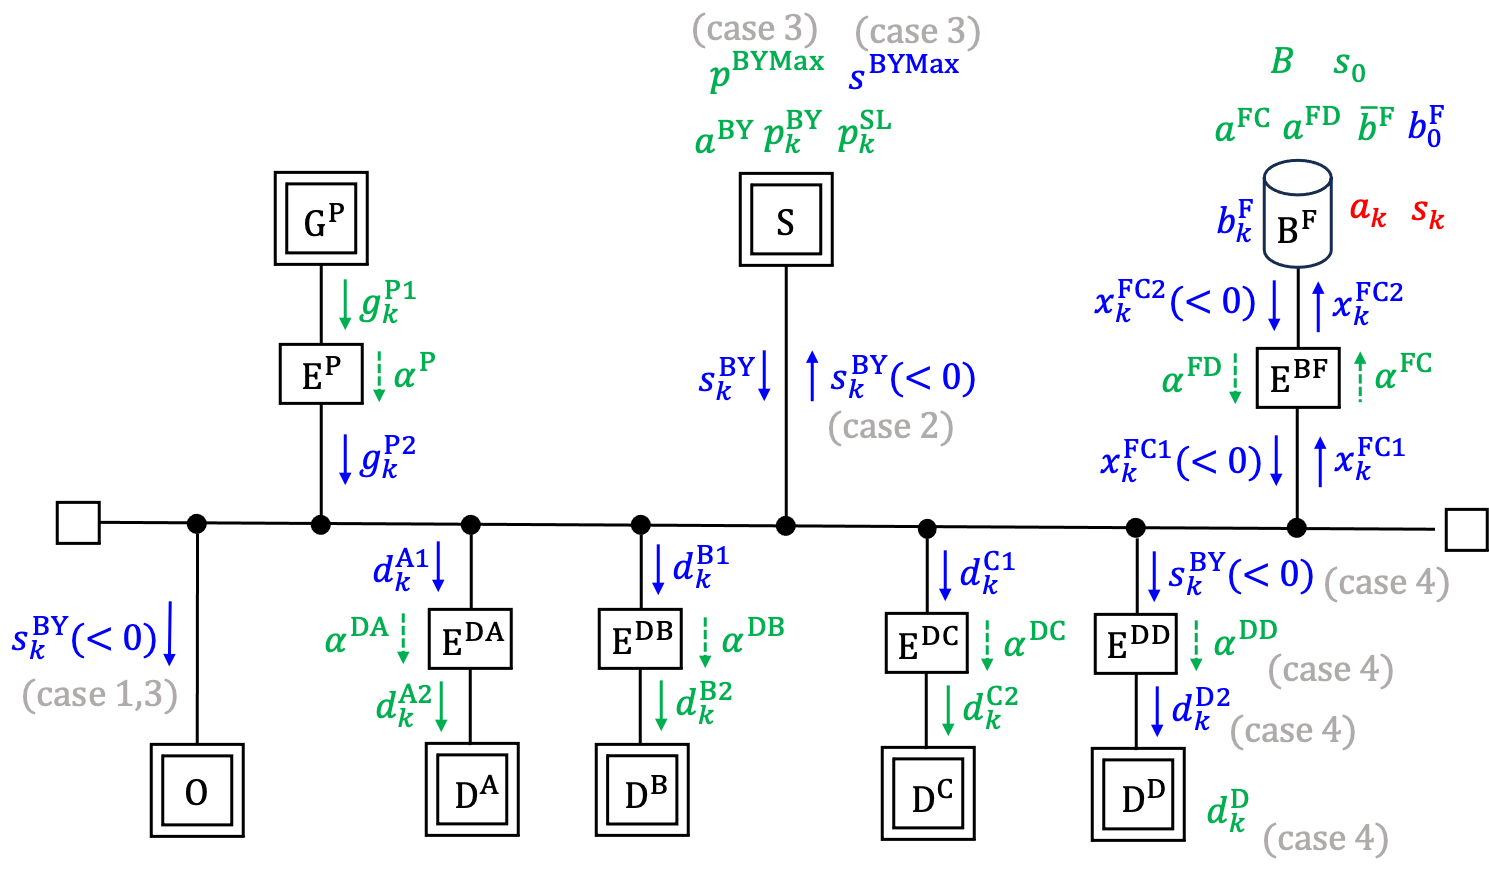
\includegraphics[width=140mm]{../figure/variables_dp.png}
 \caption{Configuration diagram of the target system(Dynamic Programming)}
 \label{fig:variables_dp}
\end{figure}

\section{定数・変数どうしの関係式}
\begin{itemize}
	\item 動線\\
		流入する電力と流出する電力の総和が等しいものとする．
		\begin{equation}
 			s_k^{\rm BY}(s_{k-1},a_{k})= 
	 		d_k^{\rm A1}+ d_k^{\rm B1} + d_k^{\rm C1}+  x_k^{\rm FC1}(s_{k-1},a_{k}) - g_k^{\rm P2},  \quad k=1,\ldots,K
 		 \label{eq:line_dp}
		\end{equation}
	\item 蓄電池\\
		蓄電池の残量は常に定められた範囲内を外れないこと，なおかつ，単位時間あたりの充放電電力は，最大出力を超過しないこと．
		\begin{equation}
       		 \label{eq:line_action_restrict}
        		\begin{split}
            		& a_k \in A_k(s_{k-1}), \\
            		& A_k(s_{k-1}) = \{ s_{k-1} + \Delta s_k^{\mathrm{Min}}(s_{k-1}),s_{k-1} + \Delta s_k^{\mathrm{Min}}(s_{k-1})+1, \dots, s_{k-1} + \Delta s_k^{\mathrm{Max}}(s_{k-1}) \},\\
            		& k=1,\dots,K
        		\end{split}
    		\end{equation}
    		ここで，$\Delta s_k^{\mathrm{Min}}(s_{k-1})$ および $\Delta s_k^{\mathrm{Max}}(s_{k-1})$ は，
		それぞれ状態 $s_{k-1}$ において許容される残量の最大放電量および最大最大充電量に相当する，添字を返す関数である．
		
		
	\item 電力変換装置\\
		パワーコンディショナや変圧器などを介して電力を変換・送電する際，一定の変換効率に応じた電力損失が発生するものとする．
		\begin{equation}
 			g^{\rm P2}_{k} = \alpha^{\rm P} g^{\rm P1}_{k} ,  \quad k=1,\ldots,K
		\label{eq:gP1gP2_dp}
		\end{equation}
		%
		\begin{equation}
 			d^{\rm A2}_{k} = \alpha^{\rm DA} d^{\rm A1}_{k} ,\quad k=1,\ldots,K
		 \label{eq:dA1A2_dp}
		\end{equation}
		%
		\begin{equation}
 			d^{\rm B2}_{k} = \alpha^{\rm DB} d^{\rm B1}_{k},\quad k=1,\ldots,K
 		\label{eq:dB1B2_dp}
		\end{equation}
		%
		\begin{equation}
 			d^{\rm C2}_{k} = \alpha^{\rm DC} d^{\rm C1}_{k},\quad k=1,\ldots,K
 		\label{eq:dC1C2_dp}
		\end{equation}
		%
		\begin{equation}
 			x^{\rm FC2}_{k}(s_{k-1},a_{k}) =\begin{cases}
  			\alpha^{\rm FC}x^{\rm FC1}_{k}(s_{k-1},a_{k})  \quad \text{if } a_k-s_{k-1} \ge 0 \\
 			 \frac{1}{\alpha^{\rm FD}}x^{\rm FC1}_{k}(s_{k-1},a_{k}) \quad \text{otherwise }
			 \end{cases},
  			\quad k=1,\ldots,K
 		\label{eq:xFC1FC2_dp}
		\end{equation}

		%
		ケース4において$s^{\rm BY}_{k} < 0$を満たす場合
		\begin{equation}
 			d^{\rm D2}_{k} = -\alpha^{\rm DC} s^{\rm BY}_{k}(s_{k-1},a_{k}),\quad k=1,\ldots,K
 		\label{eq:dD1D2_dp}
		\end{equation}
	
\end{itemize}

\section{評価関数と目的関数}
	第3章の目的関数と対応させるべく，本モデルにおける最適化の目的は，全期間を通じた電力運用コストを最小化することとする．
	これを動的計画法で扱うために，各期間ごとに発生するコストを「評価関数」として定義し，
	その総和を最小化する問題として定式化する．
	蓄電池の残量の状態 $s_{k-1}$において行動$a_{k}$を行なった際の評価関数を$R_k(s_{k-1},a_{k})$とする．
	この評価関数は，制約条件を満たす行動 $a_k \in A_{k}(s_{k-1})$ が選択されたときにのみ定義される．
	蓄電池の残量の状態や行動，状態遷移，評価関数の関係を可視化したものを図\ref{fig:network}に示す．
	このとき，目的関数は
	\begin{figure}[h]
 		\centering
 		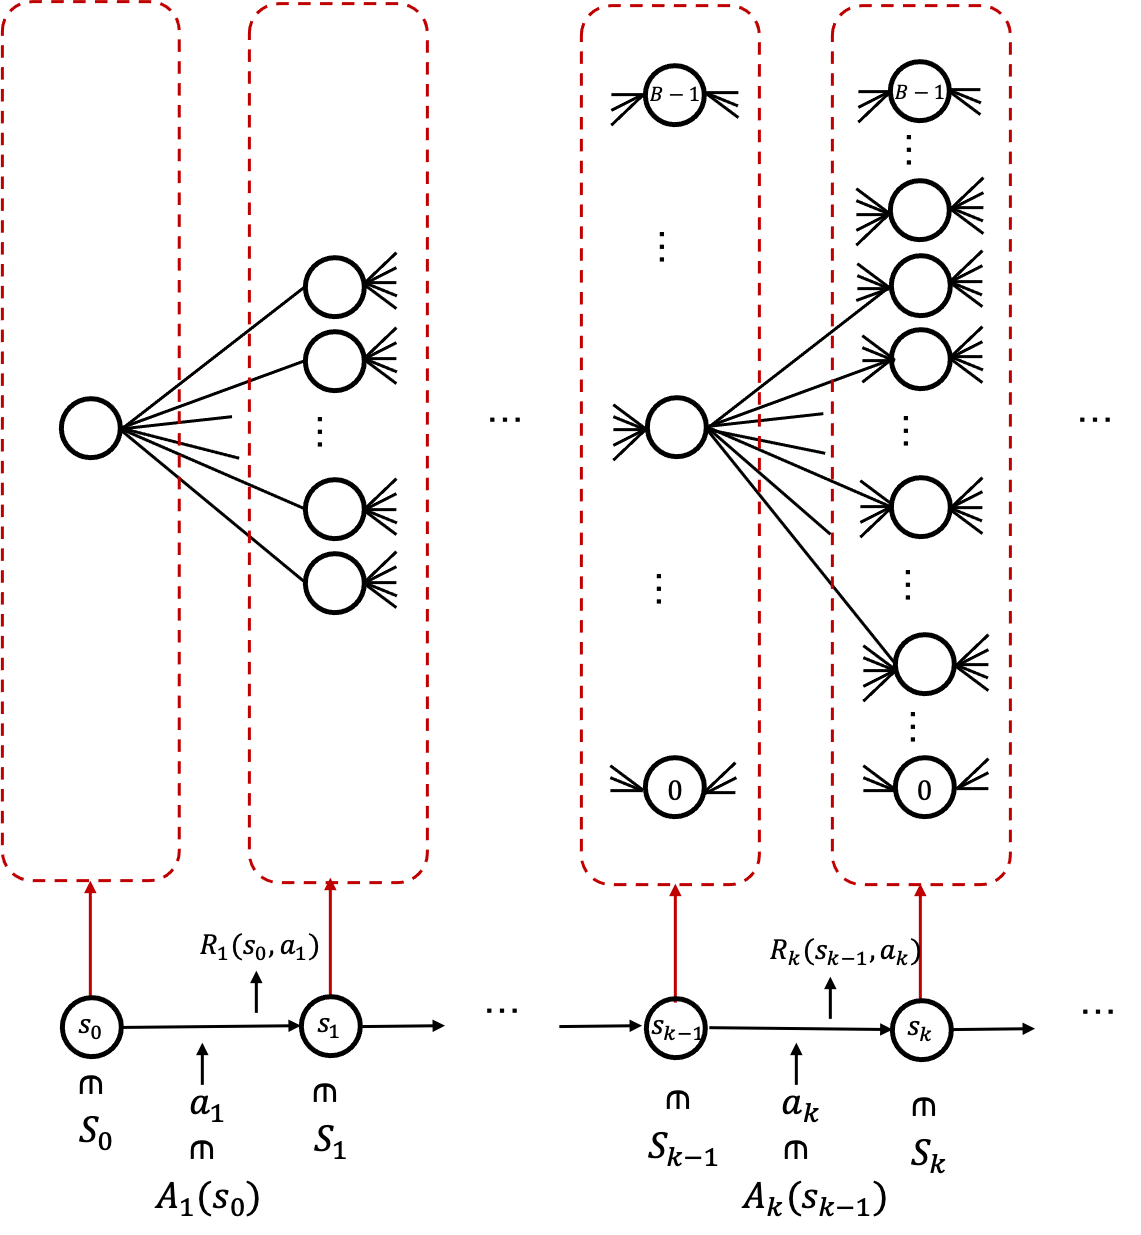
\includegraphics[width=145mm]{../figure/network.png}
 		\caption{image of state transition}
		 \label{fig:network}
	\end{figure}

	\begin{equation}
		\text{Minimize} \quad  \sum_{k=1}^{K-1} R_k(s_{k-1},a_{k}) \quad  a_{k}\in A_k({s_{k-1})}
 	\label{eq:minimize_dp}
	\end{equation}
	と表される．
	以下，評価関数の定式化の方法について述べる．評価関数の定義にはいくつかの方法が考えられるが，
	本節では3.3節で示した目的関数と対応させる形でケース1，ケース2，およびケース4の評価関数を定式化する．
	なおケース3については，0期から現在の期までの買電量の最大値を記憶しておかなければならず，最適性の原理を満足する形で定式化を行う際は
	状態空間の次元を拡張する必要があり，時間的計算量が膨大になる．よってこのケースについては本研究の対象外とするが，
	ケース3の時間的計算量についての考察は付録に記載する．

\subsection{ケース1の場合}\label{sec:R}
	$s^{\rm BY}_{k}(s_{k-1},a_{k}) < 0$を満たしているときは$|s^{\rm BY}_{k}(s_{k-1},a_{k})|$だけ無駄電力が生ずるとする
	点に注意すると，評価関数は以下のように表される：

	\begin{equation}
		R_k(s_{k-1},a_{k}) = p_k^{\rm BY} \max (s_k^{\rm BY}(s_{k-1},a_{k}) , 0).
 		\label{eq:R_1}
	\end{equation}	
	このケースでは売電を考慮しないため$s_k^{\rm BY}(s_{k-1},a_{k})$が負となる場合，
	$\max (s_k^{\rm BY}(s_{k-1},a_{k}) , 0)$の値は0となる．
	
	ここで，式\eqref{eq:line_dp}より，式\eqref{eq:R_1}は次のように書き換えられる：
	\begin{equation}
		R_k(s_{k-1},a_{k}) = p_k^{\rm BY} \max (d_k^{\rm A1}+ d_k^{\rm B1} + d_k^{\rm C1}+  x_k^{\rm FC1}(s_{k-1},a_{k}) - g_k^{\rm P2} , 0).
 		\label{eq:R_1_2}
	\end{equation}	
	また，式\eqref{eq:xFC1FC2_dp}より式\eqref{eq:R_1_2}は次のように表される．
	\begin{equation}
		R_k(s_{k-1},a_{k}) = p_k^{\rm BY} \max (d_k^{\rm A1}+ d_k^{\rm B1} + d_k^{\rm C1}+  \frac{x_k^{\rm FC2}(s_{k-1},a_{k})}{\alpha^{\rm FC}} - g_k^{\rm P2} , 0).
 		\label{eq:R_1_3}
	\end{equation}	
	ところで，式\eqref{eq:B_K}より$x_k^{\rm FC2}(s_{k-1},a_{k})$は
	\begin{equation}
		x_k^{\rm FC2}(s_{k-1},a_{k}) = (a_{k} - s_{k-1})\Delta b^{\rm F}
		\label{eq:FC2_state}
	\end{equation}
	と表され，この式\eqref{eq:FC2_state}を用いることで式\eqref{eq:R_1_3}は次のように表される：
	\begin{equation}
		R_k(s_{k-1},a_{k}) = p_k^{\rm BY} \max (d_k^{\rm A1}+ d_k^{\rm B1} + d_k^{\rm C1}+  \frac{(a_{k} - s_{k-1})\Delta b^{\rm F}}{\alpha^{\rm FC}} - g_k^{\rm P2} , 0).
 		\label{eq:R_1_4}
	\end{equation}		
	\eqref{eq:R_1_4}の右辺に含まれる $p_k^{\rm BY},d_k^{\rm B1},d_k^{\rm C1},\Delta b^{\rm F},\alpha^{\rm FC},g_k^{\rm P2}$は
	外生変数なので，遷移可能な全ての状態遷移について評価関数を設定することができる．
	
\subsection{ケース2の場合}
$s^{\rm BY}_{k}(s_{k-1},a_{k}) < 0$を満たしているときは$|s^{\rm BY}_{k}(s_{k-1},a_{k})|$だけ系統に売電するとする点に注意すると，
評価関数は以下のように表される：

\begin{equation}
  %w_{k-1}(s_{i},s_{j}) = p_k^{\rm BY/SL} \left[ \frac{j - i}{n-1} \cdot \overline{b} - \{ g_k^{\rm P2} - (d_k^{\rm A2} + d_k^{\rm B2} + d_k^{\rm C2}) \} \right]．
  %s_k^{\rm{BYMinIDX}} \le j-i \le s_k^{\rm{BYMaxIDX}}
  R_{k}(s_{k-1},a_{k}) = \begin{cases}
   p_k^{\rm BY}s_k^{\rm BY}(s_{k-1},a_{k}),\quad   \text{if } s_k^{\rm BY}(s_{k-1},a_{k}) \ge 0\\
   -p_k^{\rm SL}s_k^{\rm BY}(s_{k-1},a_{k}),\quad \text{otherwise}．
   \end{cases}
 \label{eq:R_2}
\end{equation}

この式\eqref{eq:R_2}に対して\ref{sec:R}節と同様の方法で変形を施すと次のようになる：
\begin{equation}
	R_{k}(s_{k-1},a_{k}) = \begin{cases}
	  p_k^{\text{BY}} \{d_k^{\text{A1}}+ d_k^{\text{B1}} + d_k^{\text{C1}}+  \frac{(a_{k} - s_{k-1})\Delta b^{\text{F}}}{\alpha^{\text{FC}}} - g_k^{\text{P2}} \} \\
	  \hfill \text{if } d_k^{\text{A1}}+ d_k^{\text{B1}} + d_k^{\text{C1}}+  \frac{(a_{k} - s_{k-1})\Delta b^{\text{F}}}{\alpha^{\text{FC}}} - g_k^{\text{P2}}  \ge 0 \\[1ex]
	  -p_k^{\text{SL}} \{d_k^{\text{A1}}+ d_k^{\text{B1}} + d_k^{\text{C1}}+  \alpha^{\text{FD}}(a_{k} - s_{k-1})\Delta b^{\text{F}} - g_k^{\text{P2}} \} \\
	  \hfill \text{otherwise.}
	\end{cases}
\label{eq:R_2_1}
\end{equation}
\eqref{eq:R_2_1}の右辺に含まれる $p_k^{\rm BY},d_k^{\rm B1},d_k^{\rm C1},\Delta b^{\rm F},\alpha^{\rm FC},\alpha^{\rm FD},g_k^{\rm P2}$は
	外生変数なので，遷移可能な全ての状態遷移について評価関数を設定することができる．
	
\subsection{ケース4の場合}
$s^{\rm BY}_{k}(s_{k-1},a_{k}) < 0$を満たしているときは$|s^{\rm BY}_{k}(s_{k-1},a_{k})|$だけ自己託送をするとする点に注意すると，
評価関数は以下のように表される．
\begin{equation}
  %w_{k-1}(s_{i},s_{j}) = p_k^{\rm BY/SL} \left[ \frac{j - i}{n-1} \cdot \overline{b} - \{ g_k^{\rm P2} - (d_k^{\rm A2} + d_k^{\rm B2} + d_k^{\rm C2}) \} \right]．
  %s_k^{\rm{BYMinIDX}} \le j-i \le s_k^{\rm{BYMaxIDX}}
  	R_{k}(s_{k-1},a_{k}) = \begin{cases}
   		p_k^{\rm BY}s_k^{\rm BY}(s_{k-1},a_{k}),\quad   \text{if } s_k^{\rm BY}(s_{k-1},a_{k}) \ge 0\\
   		-p_k^{\rm D}d_k^{\rm D2} ，\text{otherwise}．
  	\end{cases}
 \label{eq:R_3}
\end{equation}
式\eqref{eq:dD1D2_dp}より式\eqref{eq:R_3}は次のように書き換えられる：
\begin{equation}
  %w_{k-1}(s_{i},s_{j}) = p_k^{\rm BY/SL} \left[ \frac{j - i}{n-1} \cdot \overline{b} - \{ g_k^{\rm P2} - (d_k^{\rm A2} + d_k^{\rm B2} + d_k^{\rm C2}) \} \right]．
  %s_k^{\rm{BYMinIDX}} \le j-i \le s_k^{\rm{BYMaxIDX}}
  	R_{k}(s_{k-1},a_{k}) = \begin{cases}
   		p_k^{\rm BY}s_k^{\rm BY}(s_{k-1},a_{k}),\quad   \text{if } s_k^{\rm BY}(s_{k-1},a_{k}) \ge 0\\
   		-p_k^{\rm D}(-\alpha^{\rm DD} s^{\rm BY}_{k}(s_{k-1},a_{k})) ，\text{otherwise}．
  	\end{cases}
 \label{eq:R_3_1}
\end{equation}
この式\eqref{eq:R_3_1}に対して\ref{sec:R}と同様の方法で変形を施すと次のようになる：
\begin{equation}
R_{k}(s_{k-1},a_{k}) = \begin{cases}
    p_k^{\mathrm{BY}} \{d_k^{\text{A1}}+ d_k^{\text{B1}} + d_k^{\text{C1}}+  \frac{(a_{k} - s_{k-1})\Delta b^{\text{F}}}{\alpha^{\text{FC}}} - g_k^{\text{P2}} \} \\
    \hfill \text{if } d_k^{\text{A1}}+ d_k^{\text{B1}} + d_k^{\text{C1}}+  \frac{(a_{k} - s_{k-1})\Delta b^{\text{F}}}{\alpha^{\text{FC}}} - g_k^{\text{P2}}  \ge 0 \\[2ex]
    -p_k^{\mathrm{D}} [-\alpha^{\mathrm{DD}} \{d_k^{\text{A1}}+ d_k^{\text{B1}} + d_k^{\text{C1}}+  \alpha^{\text{FD}}(a_{k} - s_{k-1})\Delta b^{\text{F}} - g_k^{\text{P2}} \}] \\
    \hfill \text{otherwise.}
\end{cases}
\label{eq:R_3_2}
\end{equation}
\eqref{eq:R_3_2}の右辺に含まれる $p_k^{\rm BY},d_k^{\rm B1},d_k^{\rm C1},\Delta b^{\rm F},\alpha^{\rm FC},\alpha^{\rm FD},\alpha^{\rm DD},g_k^{\rm P2}$は
	外生変数なので，遷移可能な全ての状態遷移について評価関数を設定することができる．


\section{最適性の原理}
	問題を動的計画法で解くためには，目的関数が分離可能性と単調性を満たせばよい\cite{h}．
	分離可能性とは，$i$番目から$n$番目までの引数のみに依存する目的関数を$F_i(r_i,\dots,r_n)$
	としたときに，その目的関数が
	\begin{equation}
		F_i(r_i,\dots,r_n) = F_i(r_i,f_{i+1}(r_{i+1},\dots,r_n))
		\label{eq:dp_bunri}
	\end{equation}
	と表されることを指す．単調性とは，$F_i(r_i,F_{i+1})$が$F_{i+1}$に関して単調であることを表す．
	
	以下，本問題がこれらの性質を満たすことを示す．
	 本問題における目的関数を，評価関数の引数を省略して$F_{0}(R_0,R_1,\dots,R_{K})$と表すことにする．
	このとき，この目的関数の部分和である，$i$期から$K$期までの評価関数の累積和を$F_{i}(R_i,R_{i+1},\dots,R_{K})$と表すことにすると，
	\begin{equation}
		F_{i}(R_i,R_{i+1},\dots,R_{K}) = R_i+ R_{i+1}+\dots+R_{K}
		\label{eq:F_i}
	\end{equation}
	となる．式\eqref{eq:F_i}は
	\begin{equation}
		F_{i}(R_i,R_{i+1},\dots,R_{K}) = R_{i} + F_{i+1}(R_{i+1},R_{i+2},\dots,R_{K})
		\label{eq:F_i2}
	\end{equation}	
	と書き換えられる．式\eqref{eq:F_i2}の右辺の形から本問題の目的関数は分離可能性を満たす．
	次に単調性について確認する．式\eqref{eq:F_i2}において，$F_{i+1}$の係数は正の定数である．
	したがって，$F_{i+1}$の値が増加すれば$F_i$の値も増加する．
	すなわち，$F_i$は$F_{i+1}$に関して単調非減少であるため，単調性を満たす．
	以上より，本問題は分離可能性と単調性を満たしており，最適性の原理が成立するため，動的計画法により解くことができる．
	
\section{Bellman方程式}
	$F_{k}^{*}(s_k)$ を，$k$期の末尾において蓄電池の残量の状態が $s_k$ であるとき，それ以降の期（$k+1$ 期から $K$ 期まで）に
	発生する評価値の累積和の最小値と定義する．すなわち，
	\begin{equation}
		F_{k}^{*}(s_{k}) = \min \sum_{l=k+1}^{K} R_l(s_{l-1}, a_{l}) \quad a_l \in A_l(s_{l-1})
	\end{equation}
	と表される．このとき，最適性の原理に基づき，$F_{k-1}^{*}(s_{k-1})$ は，
	以下のBellman方程式によって再帰的に求めることができる．
	\begin{equation}
		F_{k-1}^{*}(s_{k-1}) = \min_{a_k \in A_k(s_{k-1})} { R_k(s_{k-1}, a_k) + F_{k}^{*}(a_k) }
		\label{eq:bellman_backward}
	\end{equation}
	ただし$K$期の末尾における評価値は次のように与えられる．
	\begin{equation}
		F_{K}^{*}(s_{K}) = 0,\quad \forall s_K \in S_K
	\end{equation}
	式 \eqref{eq:bellman_backward} において，行動 $a_k$ の決定は式 \eqref{eq:state_transition_def} より蓄電池の残量の次の状態 $s_k$ の決定と等価であるため，
	右辺第2項の $F_k^{*}$ の引数は $a_k$ となっている．この方程式を $k=K$ から $1$ へと逆方向に順次適用することで，
	各時刻・蓄電池の残量の各状態における最適な行動選択と最小コストを算出できる．最終的に，初期状態 $s_0$ に対する $F_0^*(s_0)$ を求めることで，
	全期間における最小の評価値の総和が得られる．

